

%%%%%%%%%%%%%%%%%%%%%%%%%%%%%%%%%%% Introduction to ViennaCL %%%%%%%%%%%%%%%%%%%%%%%%%%%%%%%%%%%%


\begin{frame}{ }
 \begin{center}
  \Large \textbf{Introduction to \ViennaCL}
 \end{center}
\end{frame}


\begin{frame}{Introduction to \ViennaCL}

\begin{block}{What to expect}
  \begin{itemize}
   \item What is ViennaCL
   \item OpenCL
   \item History of ViennaCL
   \item Goals of ViennaCL
   \item Installation of ViennaCL
  \end{itemize}
\end{block}

\end{frame}




\begin{frame}{What Is \ViennaCL?}

\begin{block}{What is it about the Name?}
\begin{itemize}
  \item The beautiful city of \textbf{Vienna}
  \item Open\textbf{CL}
\end{itemize}
\end{block}

\vspace{3.4cm}

\end{frame}


% \begin{frame}{What Is \ViennaCL?}
% 
% \begin{block}{What is it about the Name?}
% \begin{itemize}
%   \item The beautiful city of \textbf{Vienna}
%   \item Open\textbf{CL}
% \end{itemize}
% \end{block}
% 
% {
% \centering
% 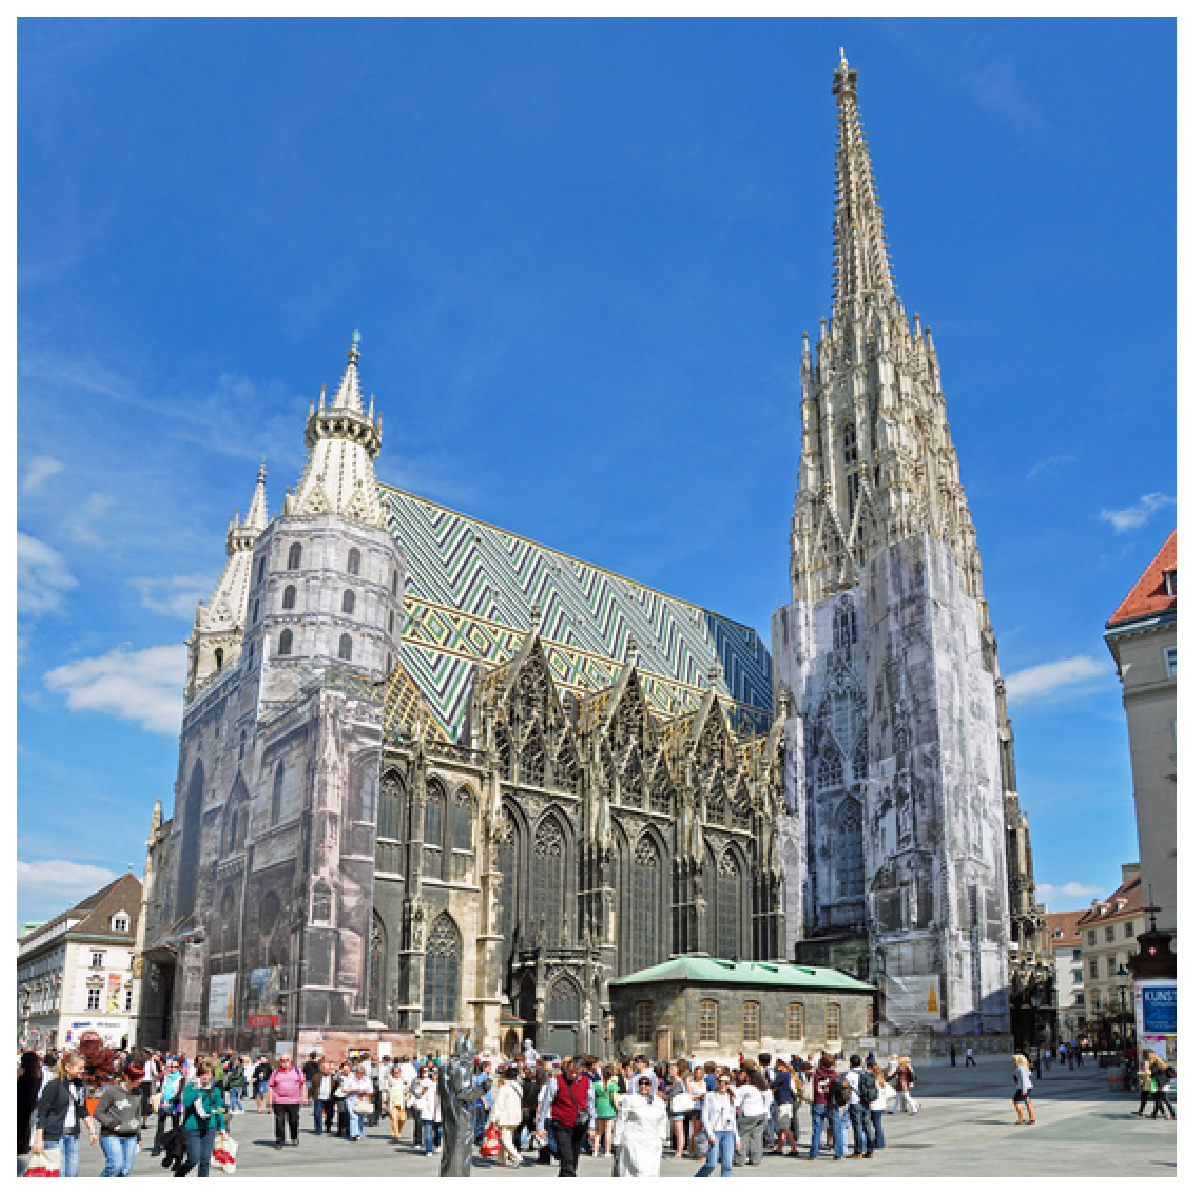
\includegraphics[width=0.3\textwidth]{figs/vienna.eps}
% }
% 
% \end{frame}


% \begin{frame}{What Is \ViennaCL?}
% 
% \begin{block}{What is it about the Name?}
% \begin{itemize}
%   \item The beautiful city of \textbf{Vienna}
%   \item Open\textbf{CL}
% \end{itemize}
% \end{block}
% 
% {
% \centering
% 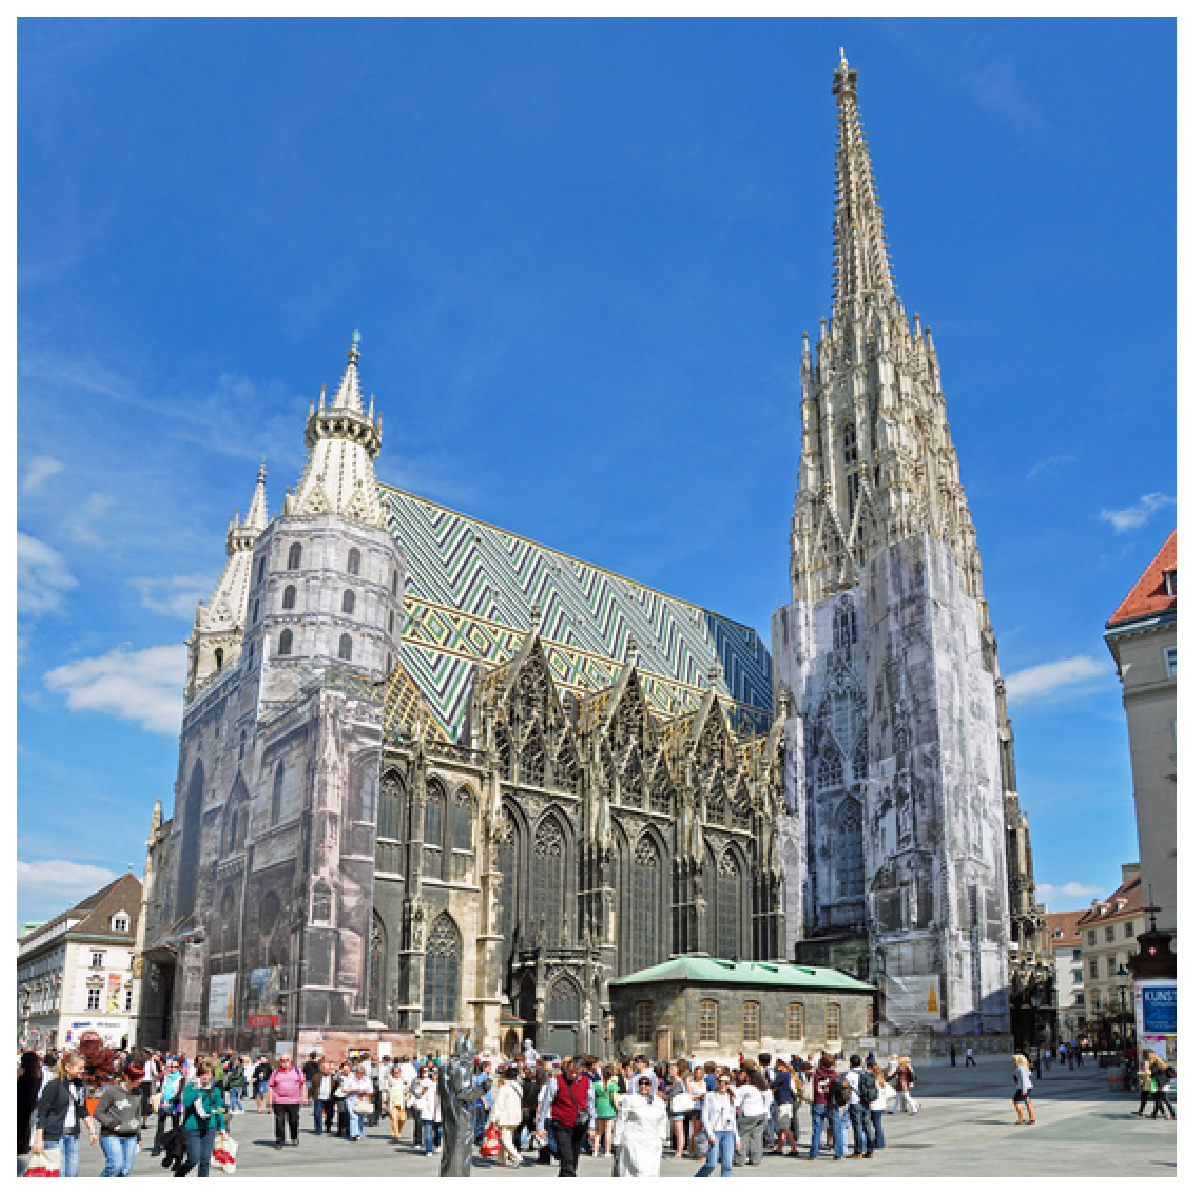
\includegraphics[width=0.3\textwidth]{figs/vienna.eps}
% \hspace{2cm}
% 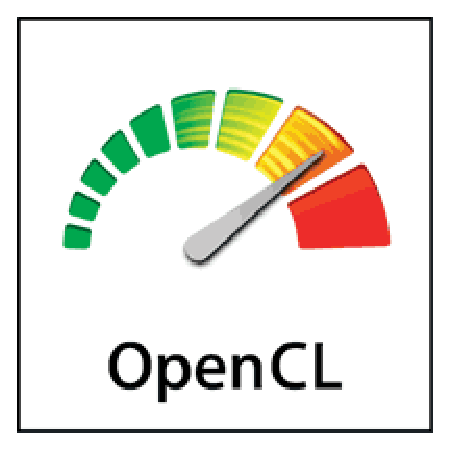
\includegraphics[width=0.3\textwidth]{figs/opencl_logo.eps}
% }
% 
% \end{frame}





\begin{frame}{History of OpenCL}

\begin{minipage}{0.6\textwidth}
\begin{block}{Prior to 2008}
  \begin{itemize}
   \item OpenCL developed by Apple Inc.
  \end{itemize}
\end{block}
\end{minipage} \hfill
\begin{minipage}{0.2\textwidth}
 
\includegraphics[width=0.99\textwidth]{figs/opencl.jpg}
\end{minipage}


\begin{block}{2008}
  \begin{itemize}
   \item OpenCL working group formed at Khronos Group
   \item OpenCL specification 1.0 released
  \end{itemize}
\end{block}

\begin{block}{2010}
  \begin{itemize}
   \item OpenCL 1.1 (multi-device, subbuffer manipulation)
  \end{itemize}
\end{block}

\begin{block}{2011}
  \begin{itemize}
   \item OpenCL 1.2 (device partitioning)
  \end{itemize}
\end{block}

\end{frame}

%%%%%%%%%%%%%%%%%%%%%%% Device %%%%%%%%%%%%%%%%%%%%%%


% \begin{frame}{OpenCL Platform Model}
%  \begin{center}
%    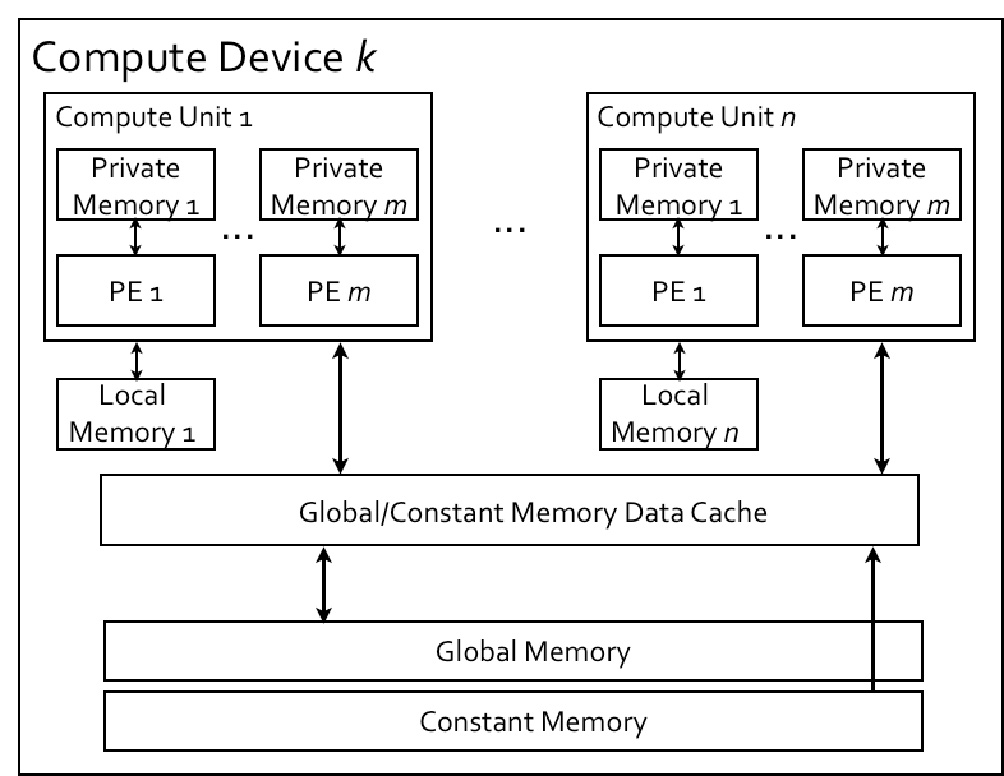
\includegraphics[width=0.8\textwidth]{figs/opencl-device.jpg} \\
%  \end{center}
%   {\tiny http://developer.amd.com/documentation/articles/PublishingImages/opencl\_figure5.jpg}
%   \vspace{0.5cm}
% \end{frame}


%%%%%%%%%%%%%%%%%%%% Platform Model %%%%%%%%%%%%%%%%%%%%%%

\begin{frame}{OpenCL Platform Model}
 \begin{center}
   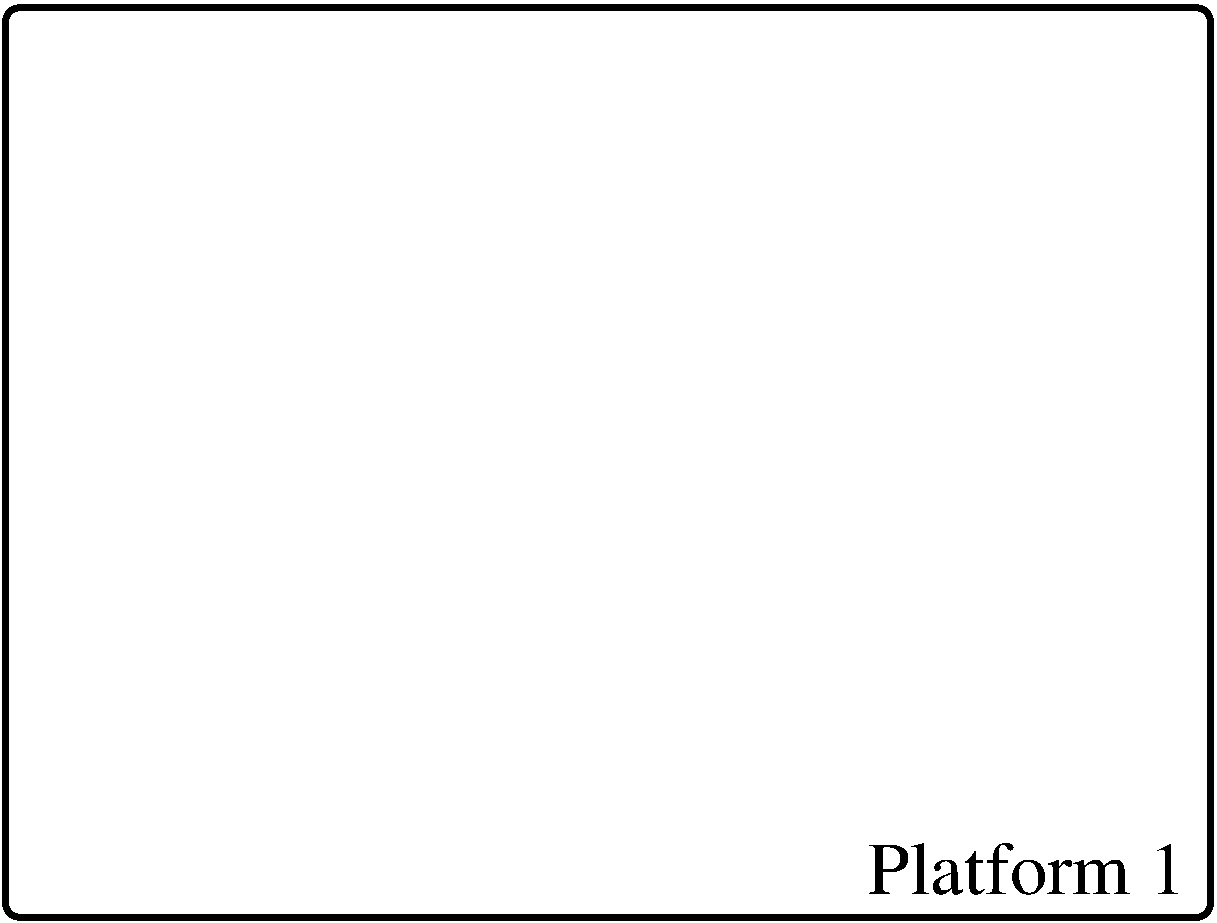
\includegraphics[width=0.85\textwidth]{figs/opencl-2.pdf}
 \end{center}
\end{frame}

\begin{frame}{OpenCL Platform Model}
 \begin{center}
   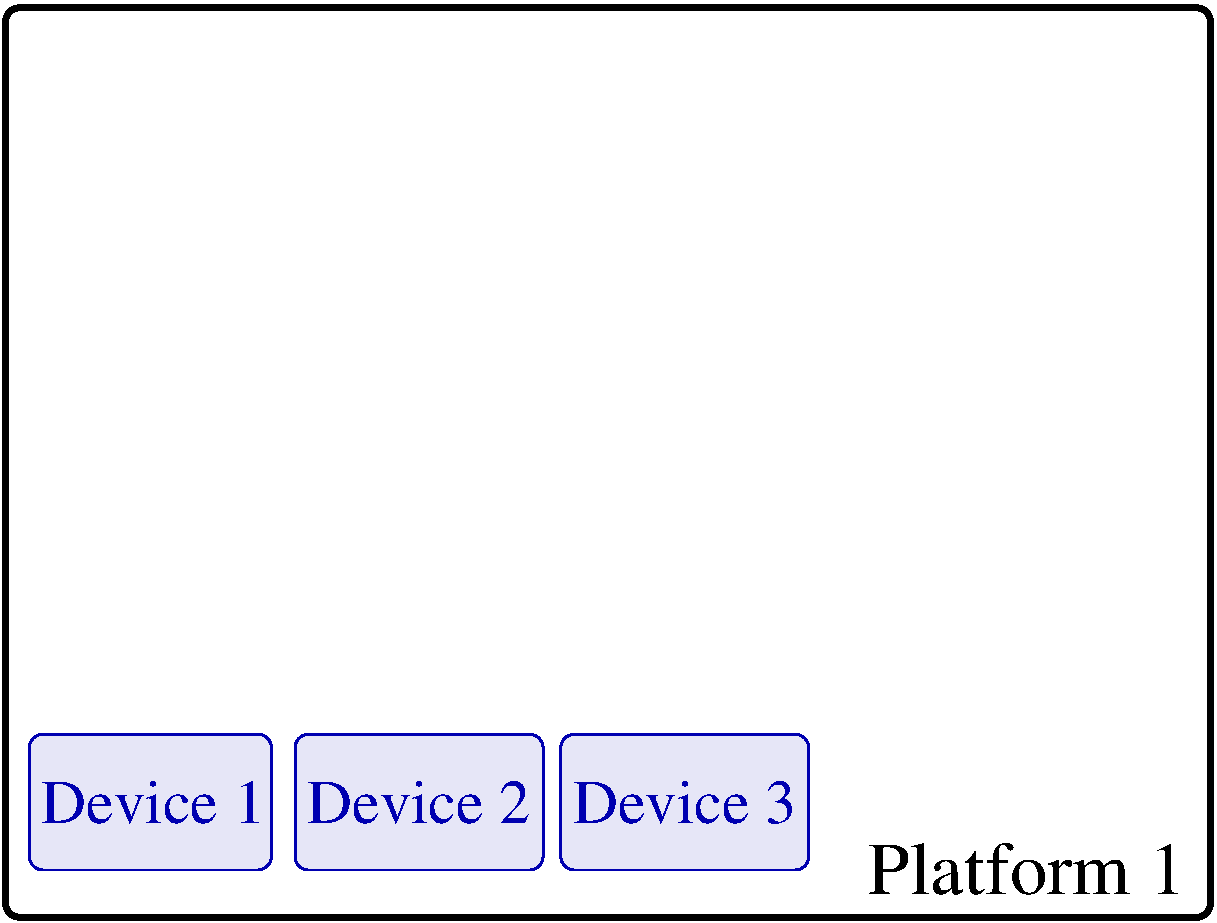
\includegraphics[width=0.85\textwidth]{figs/opencl-3.pdf}
 \end{center}
\end{frame}

\begin{frame}{OpenCL Platform Model}
 \begin{center}
   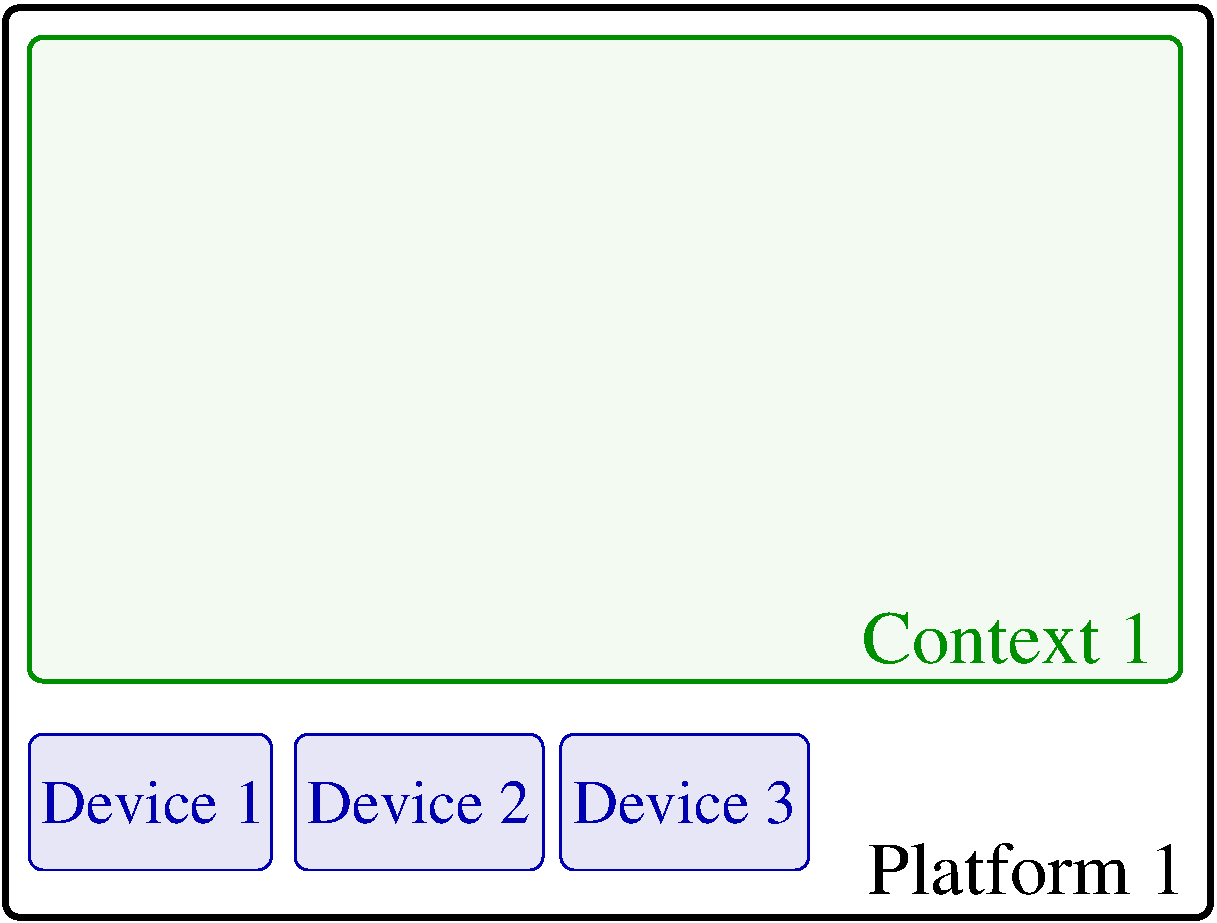
\includegraphics[width=0.85\textwidth]{figs/opencl-4.pdf}
 \end{center}
\end{frame}

\begin{frame}{OpenCL Platform Model}
 \begin{center}
   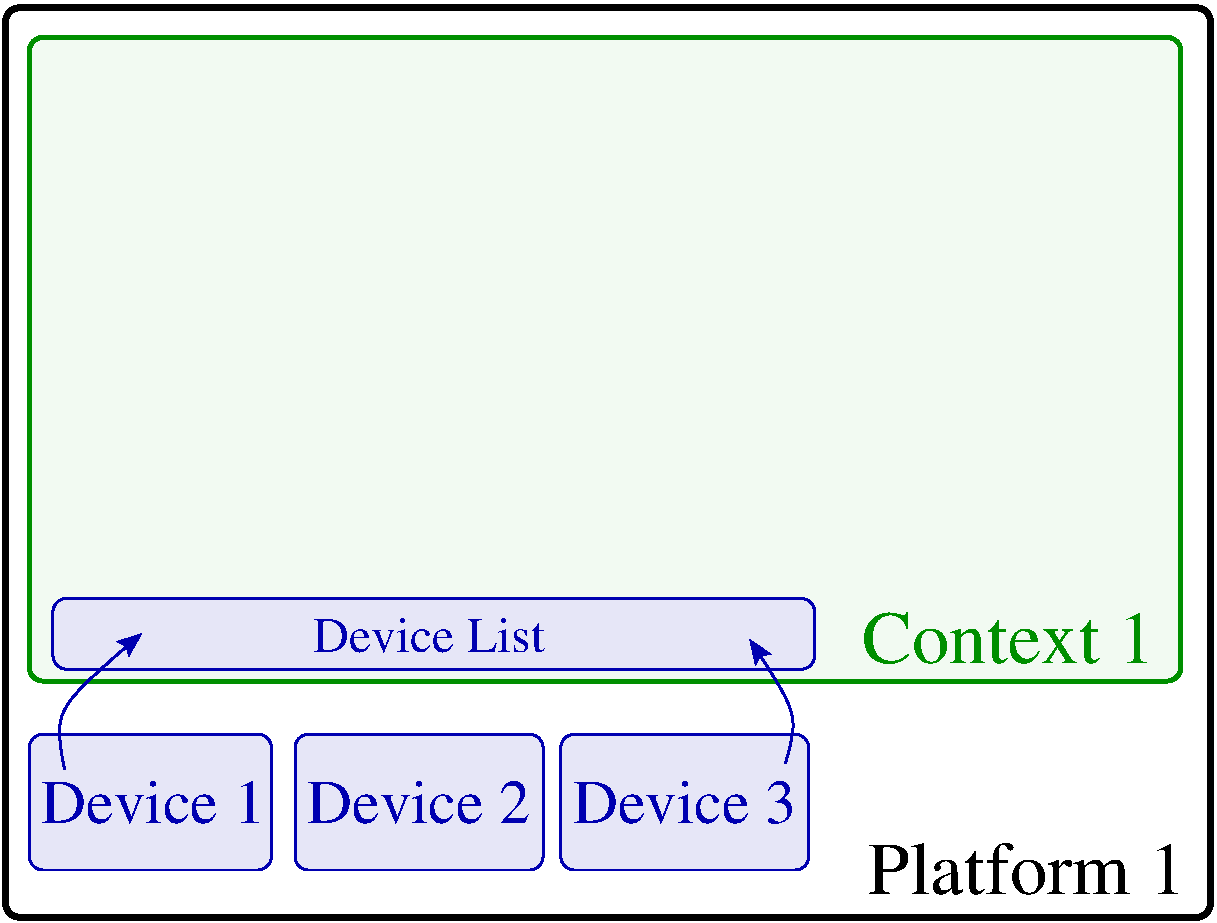
\includegraphics[width=0.85\textwidth]{figs/opencl-5.pdf}
 \end{center}
\end{frame}

\begin{frame}{OpenCL Platform Model}
 \begin{center}
   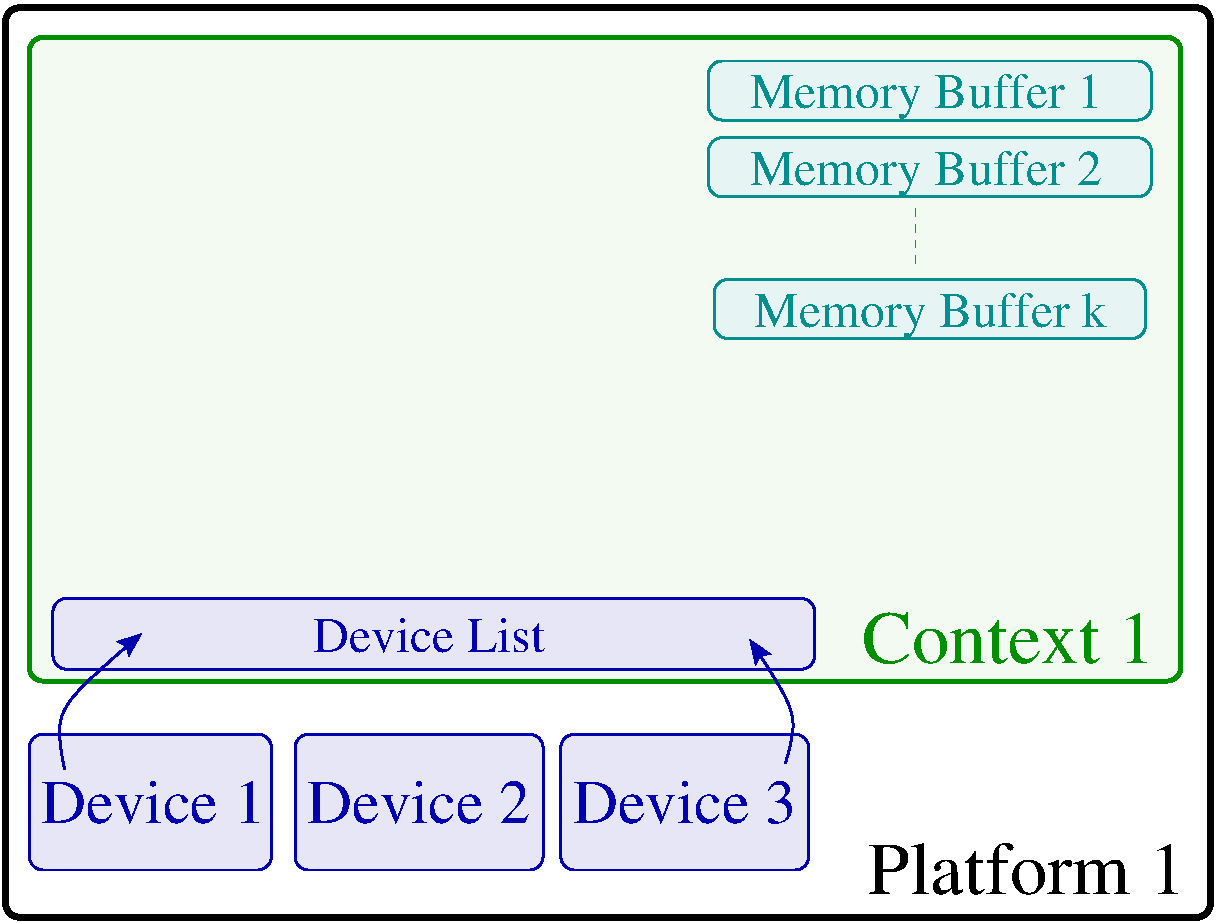
\includegraphics[width=0.85\textwidth]{figs/opencl-6.pdf}
 \end{center}
\end{frame}

\begin{frame}{OpenCL Platform Model}
 \begin{center}
   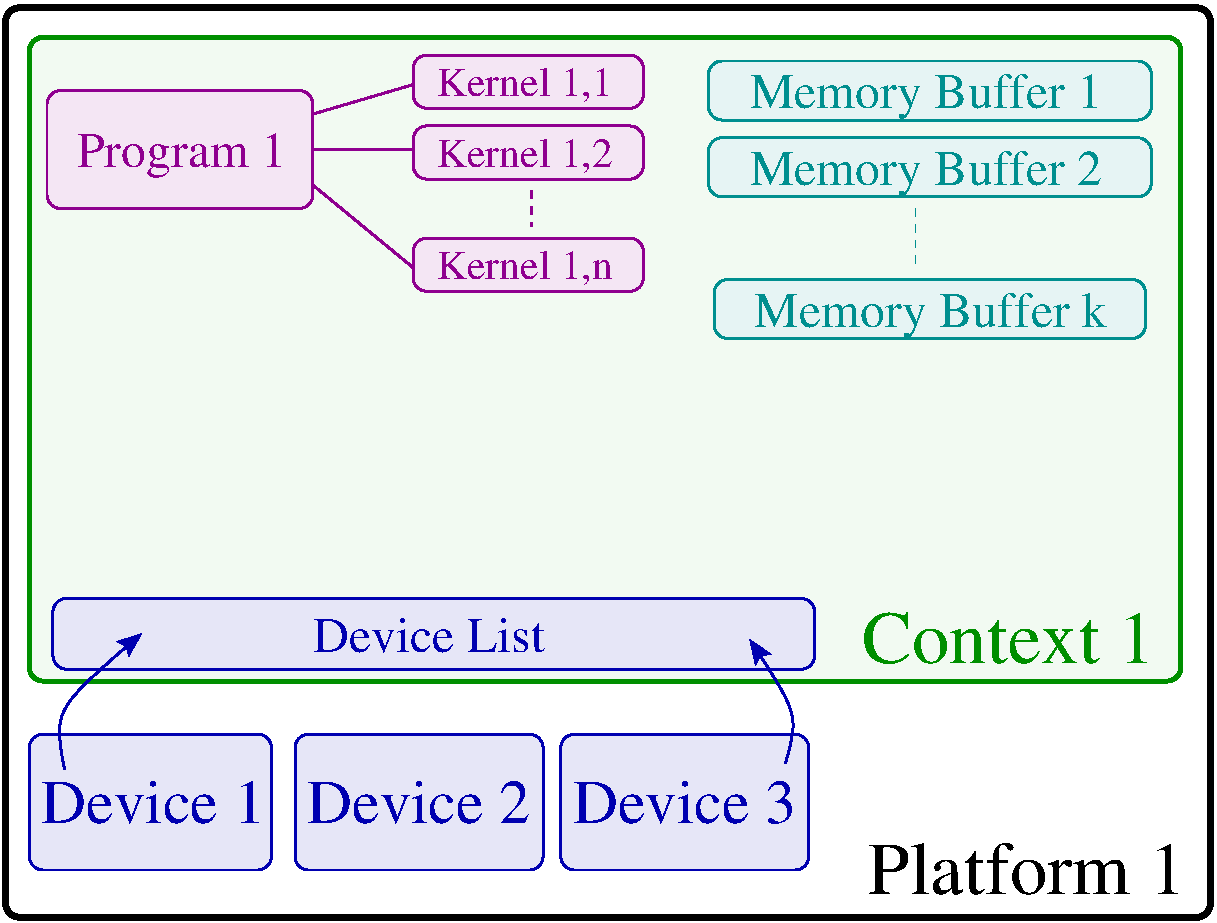
\includegraphics[width=0.85\textwidth]{figs/opencl-7.pdf}
 \end{center}
\end{frame}

\begin{frame}{OpenCL Platform Model}
 \begin{center}
   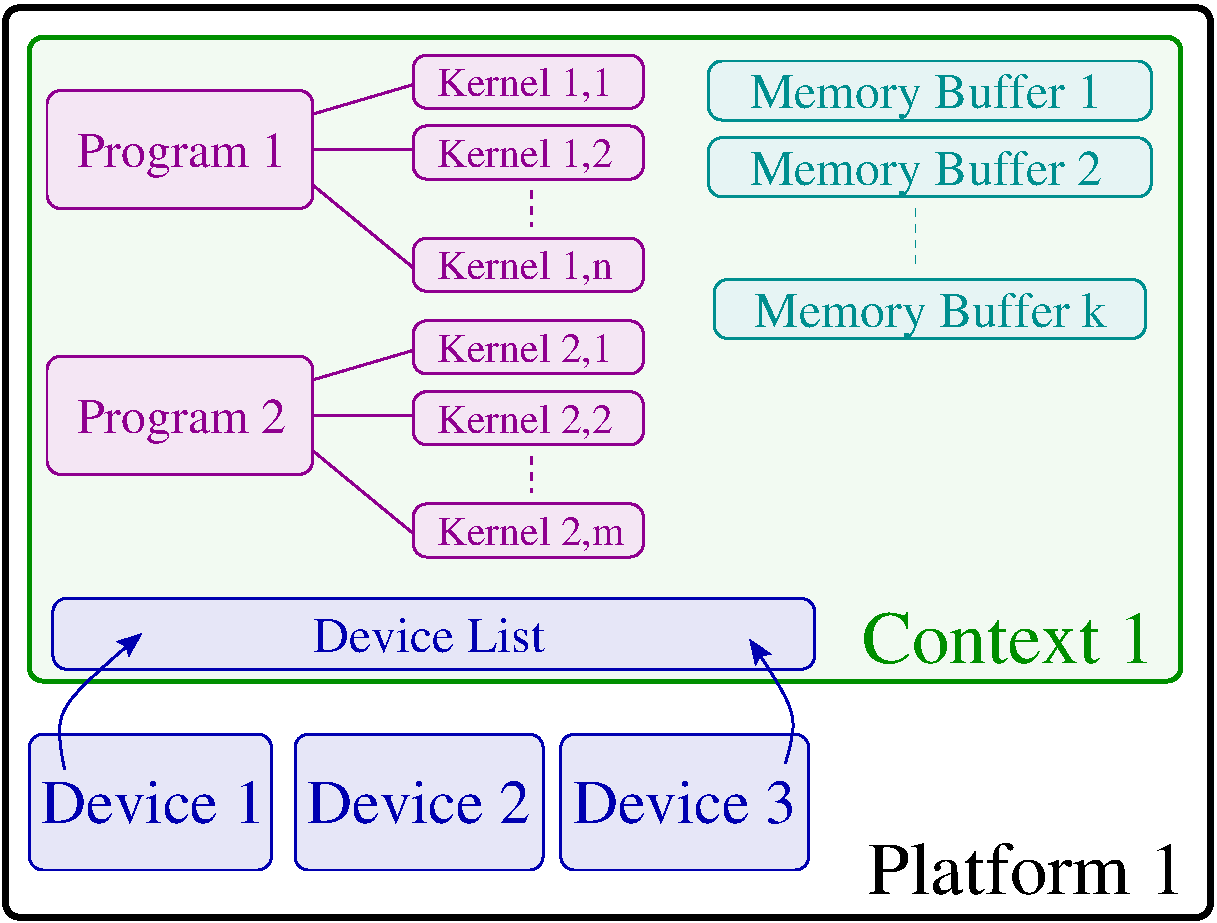
\includegraphics[width=0.85\textwidth]{figs/opencl-8.pdf}
 \end{center}
\end{frame}

\begin{frame}{OpenCL Platform Model}
 \begin{center}
   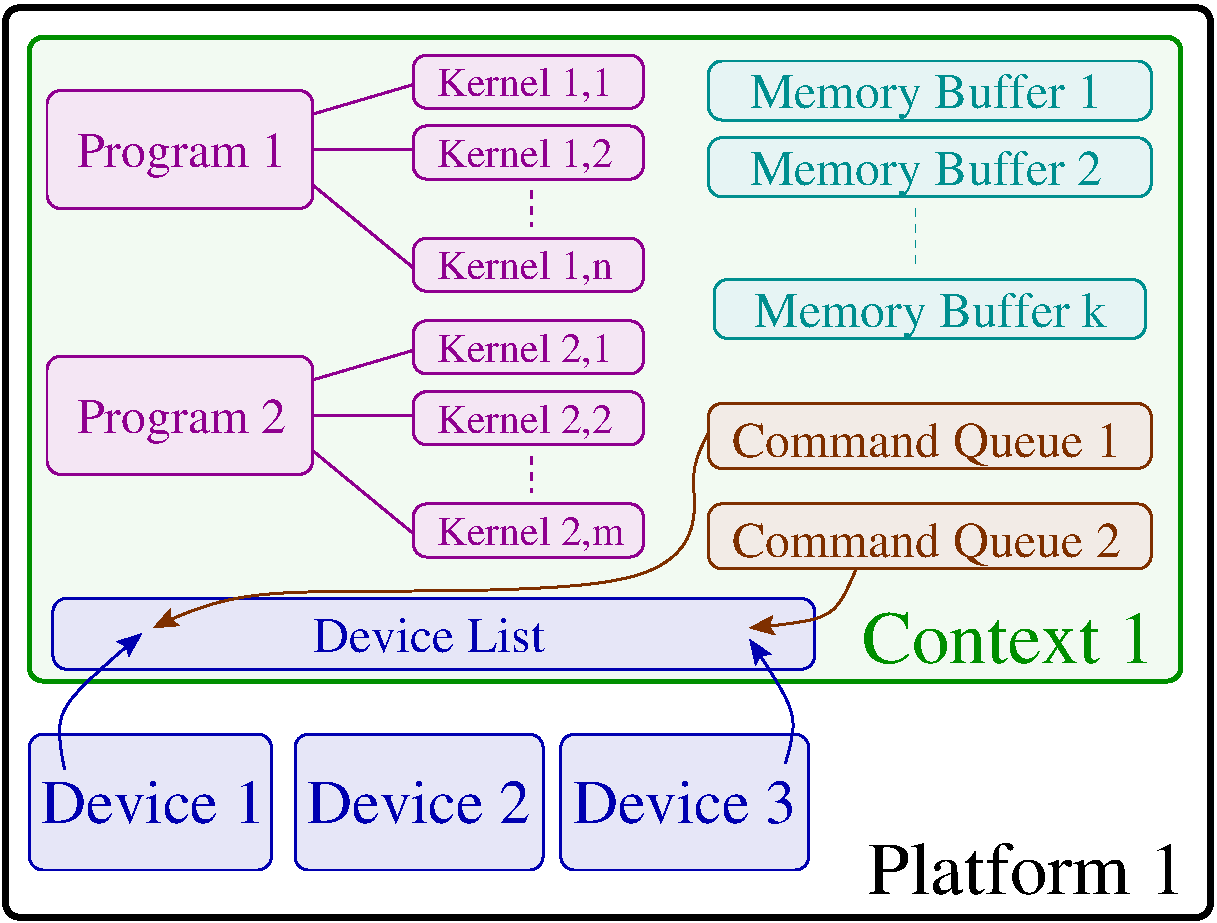
\includegraphics[width=0.85\textwidth]{figs/opencl-full.pdf}
 \end{center}
\end{frame}


%%%%%%%%%%%%%%%%%%%% Platform Model %%%%%%%%%%%%%%%%%%%%%%


\begin{frame}[fragile]
\frametitle{OpenCL Host API}

\lstset{ basicstyle=\scriptsize\ttfamily }
\begin{lstlisting}[escapechar=@]
@\color{red}{context}@ = clCreateContextFromType(NULL, CL_DEVICE_TYPE_GPU, NULL, NULL, NULL);
@\color{red}{queue}@ = clCreateCommandQueue(context, NULL, 0, NULL);
@\color{red}{memobjs[0]}@ = clCreateBuffer(context, CL_MEM_READ_WRITE, sizeof(float)*2*num_entries, NULL, NULL);
@\color{red}{memobjs[1]}@ = clCreateBuffer(context, CL_MEM_READ_ONLY | CL_MEM_COPY_HOST_PTR, sizeof(float)*2*num_entries, srcA, NULL);
 
@\color{red}{program}@ = clCreateProgramWithSource(context, 1, &kernel_src, NULL, NULL);
clBuildProgram(program, 0, NULL, NULL, NULL, NULL);
 
@\color{red}{kernel}@ = clCreateKernel(program, "my_kernel", NULL);
clSetKernelArg(kernel, 0, sizeof(cl_mem), (void *)&memobjs[0]);
clSetKernelArg(kernel, 1, sizeof(cl_mem), (void *)&memobjs[1]);
clSetKernelArg(kernel, 2, sizeof(float)*(local_work_size[0]+1)*16, NULL);
 
global_work_size[0] = 128;
 local_work_size[0] = 64;
clEnqueueNDRangeKernel(queue, kernel, 1, NULL, global_work_size, local_work_size, 0, NULL, NULL);
\end{lstlisting}
\lstset{ basicstyle=\small\ttfamily }

\begin{block}{Issues}
 \begin{itemize}
  \item ``Where is the error?''
  \item Manage OpenCL handles
 \end{itemize}

\end{block}

\end{frame}


\begin{frame}[fragile]
\frametitle{OpenCL Kernel Language}

\begin{block}{Sample Operation: Inplace Vector Addition}
 \vspace*{-0.5cm}
 \begin{align*}
  \left(
  \begin{array}{c}
   v_1^1 \\
   v_1^2 \\
   \vdots \\
   v_1^n 
  \end{array} \right) +\!= 
  \left(
  \begin{array}{c}
   v_2^1 \\
   v_2^2 \\
   \vdots \\
   v_2^n 
  \end{array} \right)
 \end{align*}
\end{block}

 \vspace*{-0.3cm}
\begin{block}{OpenCL Kernel}
\begin{lstlisting}
__kernel void inplace_add(
          __global const float * vec1,
          __global const float * vec2,
          unsigned int size) 
{ 
  for (unsigned int i  = get_global_id(0); 
                    i  < size; 
                    i += get_global_size(0))
    vec1[i] += vec2[i];
}
\end{lstlisting}
\end{block}

\end{frame}


%%%%%%%%%%%%%%%%% OpenCL closing %%%%%%%%%%%%%%%
% \begin{frame}{OpenCL Management}
%  \begin{center}
%    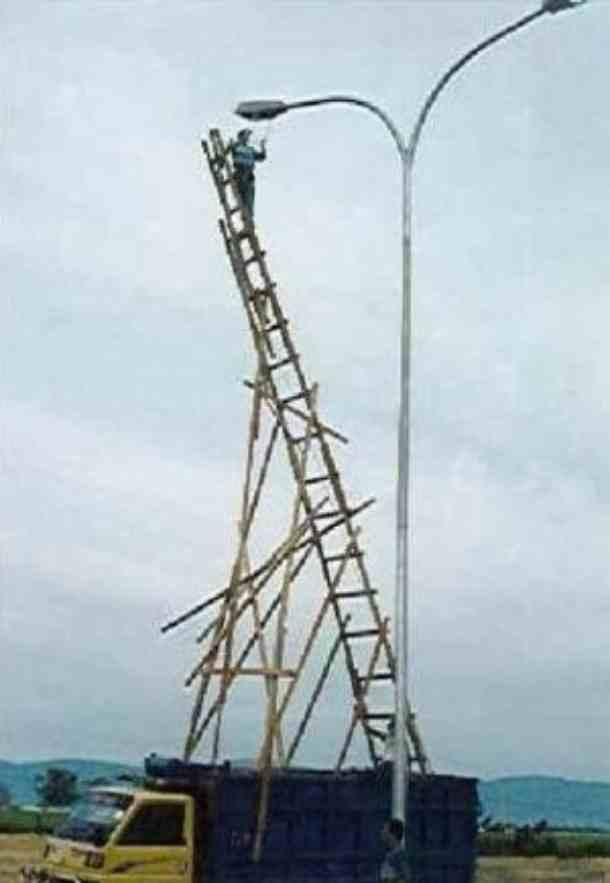
\includegraphics[width=0.45\textwidth]{figs/work1.jpg}
%  \end{center}
% \end{frame}






\begin{frame}{History of \ViennaCL}

\begin{block}{2010}
  \begin{itemize}
   \item April: Roots in the Master's Thesis of Florian Rudolf
   \item May 28th: ViennaCL 1.0.0 released
   \item November: 1000th download
   \item December: ViennaCL 1.1.0 \\(BLAS level 3, refurbished OpenCL backend)
  \end{itemize}
\end{block}

\vspace*{2.49cm}
\end{frame}



\begin{frame}{History of \ViennaCL}

\begin{block}{2010}
  \begin{itemize}
   \item April: Roots in the Master's Thesis of Florian Rudolf
   \item May 28th: ViennaCL 1.0.0 released
   \item November: 1000th download
   \item December: ViennaCL 1.1.0 \\(BLAS level 3, refurbished OpenCL backend)
  \end{itemize}
\end{block}

\begin{block}{2011}
  \begin{itemize}
   \item March: Accepted for Google Summer of Code
   \item December: ViennaCL 1.2.0 \\ (AMG, SPAI, FFT, QR, graph algorithms, structured matrices)
  \end{itemize}
\end{block}

\end{frame}



\begin{frame}{History of \ViennaCL}

\begin{block}{2012}
  \begin{itemize}
   \item March: Accepted for Google Summer of Code
   \item May: Tutorial at NVIDIA GTC 2012
   \item May: ViennaCL 1.3.0 \\ (ranges and slices, Automated OpenCL kernels, eigen values, ILU0, SVD)
   \item December: ViennaCL 1.4.0 \\ (CUDA and host backend, initializer types)
  \end{itemize}
\end{block}

\vspace{2.07cm}

\end{frame}


\begin{frame}{History of \ViennaCL}

\begin{block}{2012}
  \begin{itemize}
   \item March: Accepted for Google Summer of Code
   \item May: Tutorial at NVIDIA GTC 2012
   \item May: ViennaCL 1.3.0 \\ (ranges and slices, Automated OpenCL kernels, eigen values, ILU0, SVD)
   \item December: ViennaCL 1.4.0 \\ (CUDA and host backend, initializer types)
  \end{itemize}
\end{block}

\begin{block}{2013}
  \begin{itemize}
   \item May: Accepted for Google Summer of Code
   \item June: Tutorial at CGLibs
  \end{itemize}
\end{block}

\end{frame}


% \begin{frame}{History of \ViennaCL}
% 
% \TODO{Achievement unlocked: Historian}
% 
% \end{frame}



\begin{frame}{Goals of \ViennaCL}

  \begin{block}{About}
   \begin{itemize}
    \item High-level linear algebra C++ library
    \item OpenMP, OpenCL, and CUDA backends
    \item Header-only
    \item Multi-platform
   \end{itemize}
  \end{block}

  \vspace*{-2.3cm}
  \begin{flushright}
   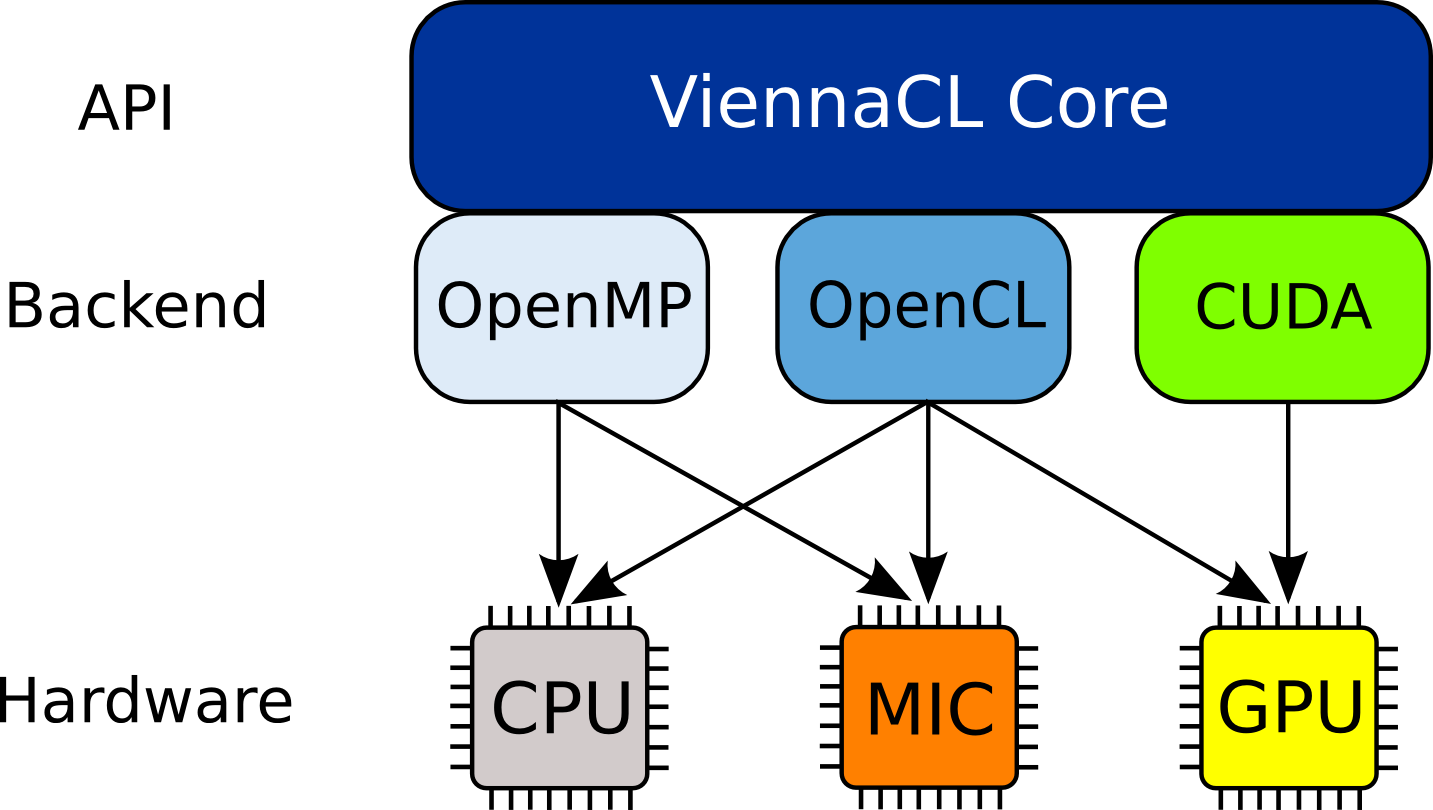
\includegraphics[width=0.4\textwidth]{figs/ViennaCL-arch.png}
  \end{flushright}

  \vspace*{-0.7cm}
  \begin{block}{Dissemination}
    \begin{itemize}
     \item Free Open-Source MIT (X11) License
     \item http://viennacl.sourceforge.net/
     \item 50-100 downloads per week
    \end{itemize}   
  \end{block}

  \begin{block}{Design Rules}
   \begin{itemize}
    \item Reasonable default values
    \item Compatible to Boost.uBLAS whenever possible 
    \item In doubt: clean design over performance
   \end{itemize}
  \end{block}

\end{frame}



\begin{frame}{Goals of \ViennaCL}

  \begin{block}{Core features}
    \begin{itemize}
     \item Linear algebra, BLAS
     \item Solver (direct and iterative)
     \item Preconditioners
    \end{itemize}   
  \end{block}
     
  \begin{block}{Additional features}
    \begin{itemize}
     \item Fast Fourier Transform
     \item Eigenvalue computations
     \item QR factorization
     \item Bandwidth reduction
     \item Nonnegative matrix factorization
    \end{itemize}   
  \end{block}

\end{frame}



\begin{frame}{Goals of \ViennaCL}

  \begin{block}{Interfaces to other libraries}
    \begin{itemize}
     \item Boost.uBLAS
     \item Eigen
     \item MTL4
    \end{itemize}   
  \end{block}

  \begin{block}{Backends}
   \begin{itemize}
    \item CPU
    \item OpenCL
    \item CUDA
   \end{itemize}
  \end{block}

  \begin{block}{C++ library}
   \begin{itemize}
    \item Generic free functions
    \item Expression templates
   \end{itemize}
  \end{block}

\end{frame}



\begin{frame}{Installation of \ViennaCL}

  \begin{block}{Three Steps}
    \begin{itemize}
     \item Download from http://viennacl.sourceforge.net/
     \item Unzip
     \item Copy source folder
    \end{itemize}   
  \end{block}

  \begin{block}{Dynamic Library?}
    \begin{itemize}
     \item ViennaCL is header-only
     \item Linking depends on used backend (OpenMP, OpenCL, CUDA)
    \end{itemize}
  \end{block}

  \begin{block}{Sample Applications}
    \begin{itemize}
     \item 22 tutorials
     \item $\hphantom{0}$7 benchmarks
     \item about 35 tests
    \end{itemize}
  \end{block}

\end{frame}

